\documentclass[a4paper,12pt]{article}
\usepackage[LY1]{fontenc}
\usepackage[utf8]{inputenc}
\usepackage{polski}
\usepackage[lf]{berenis}
\usepackage{graphicx}
\graphicspath{ {./images/} }

\DeclareTextCompositeCommand{\k}{LY1}{a}
  {\oalign{a\crcr\noalign{\kern-.27ex}\hidewidth\char7}}
\DeclareTextCompositeCommand{\k}{LY1}{e}
  {\oalign{e\crcr\noalign{\kern-.27ex}\hidewidth\char7\hidewidth}}
\DeclareTextCompositeCommand{\k}{LY1}{E}
  {\oalign{E\crcr\hidewidth\char7\hidewidth}}

\DeclareTextCompositeCommand{\'}{LY1}{c}
  {{\ooalign{\hidewidth\raise-.13875ex\hbox{\'{}}\hidewidth\crcr c}}}
\DeclareTextCompositeCommand{\'}{LY1}{s}
  {{\ooalign{\hidewidth\raise-.13875ex\hbox{\'{}}\hidewidth\crcr s}}}
\DeclareTextCompositeCommand{\'}{LY1}{z}
  {{\ooalign{\hidewidth\raise-.13875ex\hbox{\'{}}\hidewidth\crcr z}}}
\DeclareTextCompositeCommand{\'}{LY1}{C}
  {{\ooalign{\hidewidth\raise.65367ex\hbox{\'{}}\hidewidth\crcr C}}}
\DeclareTextCompositeCommand{\'}{LY1}{S}
  {{\ooalign{\hidewidth\raise.65367ex\hbox{\'{}}\hidewidth\crcr S}}}
\DeclareTextCompositeCommand{\'}{LY1}{Z}
  {{\ooalign{\hidewidth\raise.65367ex\hbox{\'{}}\hidewidth\crcr Z}}}

\begin{document}
\title{Implementacja algorytmów uczenia maszynowego do samodzielnego przechodzenia gier wideo}
\author{Kacper Majkowski}
\maketitle

\section{Motywacja}

\subsection{Historia powstania}

Uczenie maszynowe jest ostatnio bardzo popularnym tematem. Z pojawieniem się takich przydatnych technologi jak Chat GPT, lub szkodliwych jak Deepfake, widać że sztuczna inteligencja będzie grała orgomną rolę już w niedalekiej przyszłości. Ta praca skupi się na jednej dziedzinie uczenia maszynowego, mianowicie "uczenie przez wzmacnianie" (ang. "reinforcement learning / RL"). Jest to technika uczenia metodą "prób i błędów", lub dokładniej "nagród i kar". Można to lepiej przedstawić jako porównanie do tego jak uczą się ludzie i zwierzęta.

\subsection{Inspiracja naturą}

Wyobraźmy sobię mysz grasującą na małym osiedlu. Pewnego dnia wkrada się ona do domu A. Znajduje spiżarnię i dużo pysznego sera. Następnego dnia wkrada się do domu B. Tam zamiast sera znajduje groźnego kota. Mysz wie teraz że wkradanie się do domu A przynosi większą "nagrodę" niż do domu B, i powinna do niego chodzić częściej. Pojawia się jednak pewien problem. A co jeżeli w domu B kot strzeże bardziej wartościowej spiżarni niż tej w domu A? Może warto to sprawdzić, pomimo ryzyka? A może wybrać łatwiejszą opcję i chodzić cały czas do domu A? To wszystko ma swoje odzwierciedlenie w nauczaniu przez wzmacnianie.

\section{Elementy działania uczenia przez wzmacnianie}

\subsection{Nazewnictwo}

Wytłumaczenie pojęć: \newline
\newline Agent - Jednostka która wchodzi w interakcję ze środowiskiem, podejmuje decyzje oraz uczy się które decyzje są lepsze lub gorsze na podstawie otrzymanych nagród \newline
\newline Środowisko - Przestrzeń w której porusza się agent \newline
\newline Stan - Pewne unikalne warunki środowiska \newline
\newline Akcja - Decyzja podjęta przez agenta w danym stanie środowiska, prowadząca do zmiany stanu na nowy \newline
\newline Nagroda - Wartość otrzymywana przez agenta po każdej akcji, mówiąca czy wykonana akcja była właściwa czy nie \newline
\newline Epizod - Zbiór ruchów po których środowisko jest przywracane do stanu początkowego \newline
\newline Obserwacja - Zbadanie stanu przez agenta oraz ustalenie przewidywanych nagród za każdą możliwą akcję 
\newline \newline Dzięki wytłumaczeniu tych pojęć, można lepiej przedstawić na czym polega algorytm uczenia przez wzmacnianie. Na początku tworzone jest \underline{środowisko} z \underline{agentem} w \underline{stanie} wyjściowym. Następnie \underline{agent} \underline{obserwuje} obecny \underline{stan} i wykonuje \underline{akcję} na jej podstawie. Potem za wykonaną \underline{akcję} przyznawana jest \underline{nagroda}, po czym \underline{agent} wyciąga z niej wnioski. Następnie proces zaczyna się od począku: \underline{Obserwacja} -> \underline{Akcja} -> \underline{Nagroda} -> Nauka -> Nowy \underline{stan}. Jeśli \underline{agent} zakończy \underline{epizod}, \underline{stan} przywracany jest do początkowego, a \underline{agent} rozpoczyna kolejny \underline{epizod}, ale ze zdobytą już wiedzą.

\subsection{Q-Tabela}

Ale jak agent powinien zapisywać swoją wiedzę? Robi to za pomocą Tabeli, konkretnie Q-Tabeli. Przechowuje ona wszystkie kombinacje (Stan, Akcja) i zapisuje jak "opłacalna" jest to akcja w danym stanie. Nie jest to do końca nagroda za tę akcję, to trochę bardziej skomplikowane. Jak obliczamy konkretną wartość wyjaśnione będzie w kolejnym punkcie. Przykładowa Q-Tabela może wyglądać tak: \newline

\begin{center}
\begin{tabular}{ |c|c|c|c|c| }
\hline
Stan /  Akcja & Akcja 1 & Akcja 2 & Akcja 3 & Akcja 4 \\
\hline
Stan 1 & \small{1} & \small{6} & \small{-3} & \small{5} \\
\hline
Stan 2 & \small{4} & \small{1} & \small{0} & \small{-10} \\
\hline
Stan 3 & \small{-8} & \small{3} & \small{6} & \small{0} \\
\hline
Stan 4 & \small{2} & \small{0} & \small{-1} & \small{7} \\
\hline
Stan 5 & \small{0} & \small{-5} & \small{2} & \small{4} \\
\hline
\end{tabular}
\end{center}
Tutaj warto zaznaczyć że tworząc tabelę inicjalizujemy wszystkie wartości na 0, tak że zawsze mamy wartość do odczytania, nawet jeśli natrafiamy na nią po raz pierwszy. Odczytywanie tabeli jest bardzo proste. Dla przykładu jeżeli agent znajduje się w stanie 3, to z dotychczasowych doświadczeń wynika że najkorzystniejszyą akcją byłaby akcja 3. Jak jednak otrzymywać te wartości? Przy tym pomoże nam Równanie Bellmana.

\subsection{Obliczanie wartości ruchu oraz równanie Bellmana}

Równanie Bellmana pozwala nam uwzględznić wiele rzeczy które pomogą ocenić wartość danej akcji. Równanie jest dość złożone, więc zbudujmy je od podstaw. Załóżmy że właśnie wykonaliśmy akcję \(a\) w stanie \(s\) i otrzymaliśmy pewną nagrodę \(r(s, a)\):
\[ Q(s, a) =  r(s, a)\]
\(Q(s, a)\) - nowa wartość akcji w Q-Tabeli którą chcemy wyznaczyć \newline
\(r(s, a)\) - nagroda (ang. reward) za wykonanie akcji \(a\) w stanie \(s\) \newline
\newline Tak wyglądałoby równanie, gdybyśmy brali pod uwagę jedynie nagrodę za właśnie wykonaną akcję \(a\) w stanie \(s\) i nic poza tym.  \newline \newline Co jednak jeśli gorsza akcja teraz prowadzi do o wiele lepszej nagrody później? Jak uwzględnić to w równaniu? Robimy to, dodając do otrzymanej nagrody najlepszą wartość następnego ruchu po wykonaniu rozpatrywanej akcji. Innymi słowy, idziemy krok dalej i rozglądamy się, jakie akcje możemy wykonać po zrobieniu tego ruchu.

\[ Q(s, a) =  r(s, a) + \max_{a'}Q(s', a')\]
\(s'\) - Stan po wykonaniu akcji \(a\) w stanie \(s\) \newline
\(\max_{a'}Q(s', a')\) - Wartość najlepszej akcji w następnym stanie \(s'\) (maks po wszystkich możliwych akcjach)
\newline \newline Tutaj dochodzimy do jednego z kluczowych momentów. Skąd jednak mamy znać wartości ruchów w stanie \(s'\)? Tutaj z pomocą przychodzi Q-Tabela. Naiwnym podejściem byłoby rekursywne wykorzytywanie tej fromuły i zagłębiania się coraz to głębiej w drzewo możliwości. Zamiast tego odczytujemy już wcześniej wyliczoną wartość z Q-Tabeli. 
 
Aby to lepiej zrozumieć rozważmy teraz sytuację gdy wszystkie wartości w Q-Tabeli są optymalne. Skoro wiemy że wartość następnego stanu i akcji \(Q(s', a')\) również została wyliczona wcześniej za pomocą równania Bellmana, to możemy zamienić \((s', a')\) na \((r(s', a') + \max_{a''}Q(s'', a''))\). Otrzymujemy wtedy:

\[ Q(s, a) =  r(s, a) + \max_{a'}r(s', a') + \max_{a''}Q(s'', a'')\]

Tutaj otrzymujemy kolejny element \((s'', a'')\), dla którego możemy zastosować te podstawienie. Jeżeli będziemy tak kontynuować to zobaczymy że faktycznie to równanie mówi że wartość teraz to suma wszystkich kolejnych nagród, jeżeli kierujemy się zawsze najlepszymi akcjami: 
\[ Q(s, a) =  r(s, a) + \max_{a'}r(s', a') + \max_{a''}r(s'', a'') + \max_{a'''}r(s''', a''') + ...\]

Oznacza to jednak, że nagrody którą dostaniemy w przyszłości mają dla nas takie same znaczenie jak nagrodę którą dostaliśmy teraz. Nie jest to zawsze najlepsze podejście. Nasza mysz pewnie wolałaby dostać ser teraz niż na miesiąc. Dlatego tutaj wprowadzimy kolejny parametr - "współczynnik dyskontowania" (and. "discount rate"). Mówi on jak spada dla nas wartość nagród, im dalej w przyszłości je dostaniemy. Parametr ten oznaczamy grecką literą $\gamma$ (gamma). Przyjmuje on wartości od 0 do 1. Dla $\gamma = 0$ nie bierzemy przyszłych nagród pod uwagę i kierujemy się tylko natychmiastową nagrodą za ruch. Dla $\gamma = 1$, mamy sytuację jak w równaniu powyżej, gdzie przyszłe nagrody są dla nas dokładnie tak samo warte jak nagroda natychmiastowa. Wprowadzamy ten parametr do równania, dodając go jako współczynnik przy \(\max_{a'}r(s', a')\)

\[ Q(s, a) =  r(s, a) + \gamma * \max_{a'}Q(s', a')\]
\newline Teraz jeżeli wykonamy przedstawione wcześniej podstawianie otrzymujemy:
\[ Q(s, a) =  r(s, a) + \gamma * \max_{a'}r(s', a') + \gamma ^ 2 * \max_{a''}r(s'', a'') + \gamma ^ 3 * \max_{a'''}r(s''', a''') + ...\]
Oznacza to, że dla \(\gamma < 1\), każda kolejna nagroda będzie dla nas mniej wartościowa. Dla przykładu dla \(\gamma = \frac{1}{2}\) nagroda którą dostalibyśmy za 2 ruchy jest dla nas warta połowę swojej wartości, za 3 ruchy  \(\frac{1}{4}\) swojej wartości itd. 
\newline \newline To co otrzymaliśmy jest właśnie znane jako równanie Bellmana. Przedstawia ono zależności między wartościami w optymalnej Q-Tabeli. My jednak nie mamy tej optymalnej Q-Tabeli, my chcemy do niej dążyć. Robimy to, powtarzając ten proces wiele razy: Obserwacja -> Akcja -> Nagroda -> Nowy stan. 

Powinniśmy uwzględnić również wcześniejszą wiedzę o obecnej wartości \(Q(s, a)\). Gdybyśmy tego nie robili, szybkie i znaczące zmainy w Q-Tabeli mogłyby zaburzyć działanie algorytmu. Spowalniając szybkość uczenia sprawiamy, że kosztem dłuższego procesu uczenia jest ono stabilniejsze i nie dochodzi do dużych wahań. Tutaj w grę wchodzi parametr zwany "współczynnik nauczania" (ang. "learning rate"). Definiuje on jaką wagę przykładamy do nowych informacji, a jaką do już znanych. Jest on oznaczany grecką literą $\alpha$ (alfa). Współczynnik nauczania przyjmuje wartość od 0 do 1. Dla wartości 0 program nic by się nie uczył, uważał by zdobytą nagrodę za bezwartościową. Dla współczynnika 1, program zapomiałby wszystko co wcześniej wiedział od danej parze (stan, akcja), i przepisywał nową nauczoną wartość do tabeli. Ważne jest więc aby odpowiednio dobrać współczynnik nauczania pomiędzy 0 a 1, odpowiednio do naszego problemu. Dzięki niemu możemy zmodyfikować nasze równanie aby wyglądało tak:
\[ Q(s, a) =  (1 - \alpha )*Q(s, a) + \alpha * ( r(s, a) + \gamma * \max_{a'}Q(s', a') )\]
\(Q(s, a)\) - obecna wartośc dla pary (stan, akcja) w Q-Tabeli, którą chcemy poprawić \newline
\newline Po krótkim spojrzeniu można zauważyć że jest to po prostu średnia ważona obecnej wartości oraz nowej, wyliczonej za pomocą równania Bellmana, gdzie \(\alpha\) jest wagą nowej wartości a \(1-\alpha\) wagą tej z tabeli.
\newline \newline Gdy już wiemy jak uzupełniać Q-Tabelę na podstawie stanów, akcji i nagród, zobaczmy to na przykładzie wcześniej przedstawionej tabeli

\begin{center}
\begin{tabular}{ |c|c|c|c|c| }
\hline
Stan /  Akcja & Akcja 1 & Akcja 2 & Akcja 3 & Akcja 4 \\
\hline
Stan 1 & \small{1} & \small{6} & \small{-3} & \small{5} \\
\hline
Stan 2 & \small{4} & \small{1} & \small{0} & \small{-10} \\
\hline
Stan 3 & \small{-8} & \small{3} & \small{6} & \small{0} \\
\hline
Stan 4 & \small{2} & \small{0} & \small{-1} & \small{7} \\
\hline
Stan 5 & \small{0} & \small{-5} & \small{2} & \small{4} \\
\hline 
\end{tabular}
\newline
\end{center} 
Przyjmijmy również dane parametry:
\newline Współczynnik nauczania: \(\alpha = 0.3\)
\newline Współczynnik dyskontowania: \(\gamma = 0.8\)
\newline \newline Załóżmy że agent znajdował się w stanie 4 oraz podjął akcję 3. Za tę akcję otrzymał nagrodę w wysokości 5 punktów. Po wykonaniu tej akcji znalazł się w stanie 1. Oznacza to że:
\newline Stan \(s = 4\)
\newline Akcja \(a = 3\)
\newline Nagroda \(r(4, 3) = 5\)
\newline Nowy stan \(s' = 1\)
\newline \newline Wstawiając te wartości do formuły otrzymujemy: \newline
\( Q(s, a) =  (1 - \alpha )*Q(s, a) + \alpha * ( r(s, a) + \gamma * \max_{a'}(s', a') ) = (1 - 0.3)*(-1) + (0.3)*(5 + 0.8*max([1, 6, -3, 5])) = -0.7 + (0.3)*(5 + 0.8*6) = -0.7 + 2.94 = 2.24\)
\newline Tę wartość wstawiamy w pole (stan 4, akcja 3), po czym wykonujemy koleją akcję, będąc w stanie 1. Tylko jak wybrać którą akcję mamy wykonać? Najlepszą - akcję 2, aby dalej polepszać najlepsze dotąd rozwiązanie. Czy może jakąś inną, w nadzieji że znajdziemy później coś lepszego? 

\subsection{Eksploracja vs Eksploitacja}

Najlepiej byłoby gdybyśmy na początku uczenia wybierali akcje losowo (nazywamy to exploracją, ang. exploration) . Pozwoli to na przejrzenie jak najwięcej liczby stanów, aby jak najwięcej dowiedzieć się o środowisku. Jednocześnie dobrze by było gdybyśmy w późniejszej fazie częściej wybierali najlepszą odkrytą ścieżkę, aby ją dalej polepszać i otrzymywać coraz lepsze rozwiązania na jej podstawie (nazywamy to exploitacją, ang. exploitation). Tylko jak to zaimplementować?

Zastosujemy kolejny parametr, który nazwiemy "współczynnikim eksploracji" (ang. "exploration rate"). Oznaczymy go grecką literą \(\epsilon\) (epsilon). Podobnie jak pozostałe wcześniej użyte parametry, przyjmuje on wartość od 0 do 1. Jego zastosowanie jest bardzo proste - przed wyborem akcji losujemy liczbę \(x\) od 0 do 1. Jeżeli \(x\) < \(\epsilon\) wtedy wybieramy losową akcję za wszystkich możliwych, w przeciwnym wypadku wybieramy akcję o największej wartości. Można zauważyć że dla \(\epsilon = 1\) zawsze będziemy wybierać losowe akcje, dla \(\epsilon = 0\) zawsze będziemy wybierać najlepsze akcje, a dla np. \(\epsilon = 0.5\) będziemy w połowie przypadków wybierać losową akcję, a w połowie najlepszą akcję.

Ideą jest więc aby zacząć od wysokiego współczynnika eksploracji \(\epsilon\), i z czasem uczenia stopniowo go zmniejszać. Jest na to wiele sposobów ale omówimy sobie dwa - liniowy oraz geometryczny. W sposobie liniowym z każdą iteracją odejmujemy pewną wartość od współczynnika exploracji: \(\epsilon_{i+1} = \epsilon_{i} - x\), gdzie \(x =  \frac{\epsilon_{0} - \epsilon_{N}}{N}\). N to docelowa liczba iteracji podczas całego uczenia. 
\newline \newline Tak może wyglądać przykładowy wykres przedstawiający wartość współczynnika eksploracji zależnie od postępu nauczania algorytmu używając metody liniowej:
\newline 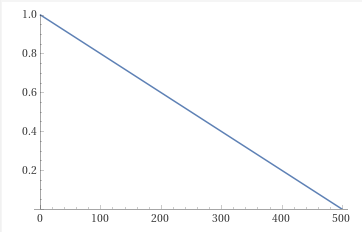
\includegraphics{lin.png}
\newline
W metodzie geometrycznej zamiast tego mnożymy współczynnik eksploracji przez pewną liczbę: \(\epsilon_{i+1} = \epsilon_{i} * x\), gdzie \(x = (\frac{e_{N}}{e_{0}})^\frac{1}{N} \). N to docelowa liczba iteracji podczas całego uczenia. 
\newline Tak wygląda przykładowy wykres dla metody geometrycznej:
\newline 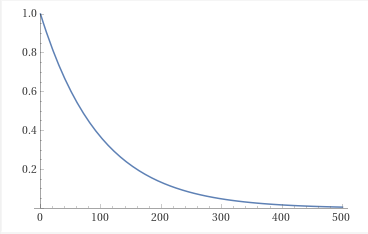
\includegraphics{geo.png}
\newline Można zauważyć że w metodzie geometrycznej dużo więcej czasu algorytm spędza z niższym współczynnikiem eksploracji. Oznacza to że szybciej porzuca strategię odkrywania środowiska i skupia się na doskonaleniu odnalezionego już rozwiązania. W przedstawionych przykładach wybrałem startowy \(\epsilon = 1\) i końcowy \(\epsilon = 0\), ale można dobrać dowolny przedział, zależnie od potrzeb i warunków środowiska.  

\section{Przedstwanienie działania uczenia przez wzmacnianie w praktyce}

\subsection{"Catch the coins"}

Sprawdźmy teraz czy ta cała teoria ma swoje odzwierciedlenie w rzeczywistości. Do tego celu posłuży nam stworzona specjalnie do tego celu gra "Catch the coins".
Pierwsza wersja gry polegała na łapaniu spadających monet. Gracz znajdował się na dole ekranu, a z góry losowo spadałyby monety. Celem gry było złapanie jak najwięcej monet w określonym czasie. Dlaczego więc zrezygnowano z tej wersji gry? Losowość.
Uczenie przez wzmacnianie bardzo słabo radzi sobie z losowością. Dlaczeo? Przypomijmy sobie jak aktualizuje się wartości w Q-Tabeli:
\[ Q(s, a) =  (1 - \alpha )*Q(s, a) + \alpha * ( r(s, a) + \gamma * \max_{a'}Q(s', a') )\]
\newline Problemem jest moment, gdy musimy "podejrzeć" najlepszą akcję w następnym stanie. Polegamy wtedy na fakcie, że w danym stanie ta sama akcja zawsze prowadzi to takiego samego stanu. Jeżeli jednak gra ma elementy losowe, nie możemy tego przewidzieć z absolutną pewnością. Z tego powodu ta metoda nie sprawdzi się w tej sytuacji. Druga wersja gry została stworzona aby nie mieć tego problemu. Innymi słowy, jest całkowicie deterministyczna.
\newline \newline
Nowa wersja gry rozgrywa się na planszy m x n. Gracz startuje w wyznaczonym miejscu na tej planszy. Na planszy znajduje się również pole wyjściowe, do którego gracz ma za zadanie dojść w jak najmniejszej liczbie kroków, poruszając się w górę, dół, prawo lub lewo jedno pole co ruch. Na planszy znajdują się również inne obiekty, mianowicie "dobre" i "złe" monety. Gracz dostaje punkty jeżeli zbierze dobrą monetę, oraz traci punkty jeżeli zbierze złą monetę. Zadaniem gracza jest więc zebranie dobrych monet, unikanie złych oraz dojście do celu w jak najmniejszej liczbie kroków.
\newline Przykładowe plansze startowe: \newline
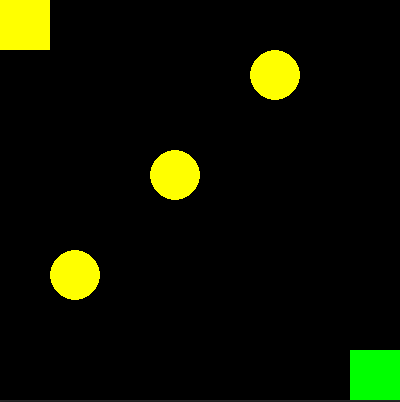
\includegraphics[width=70mm]{przyklad1.png}
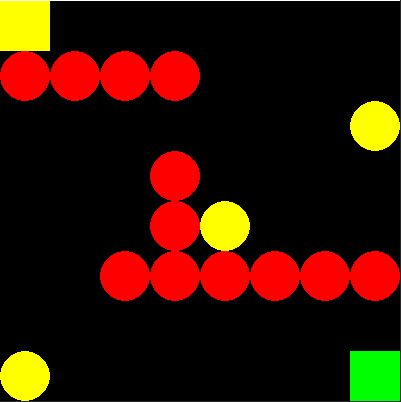
\includegraphics[width=70mm]{przyklad2.png} \newline
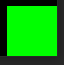
\includegraphics[width=20mm]{player.png} - Gracz (Agent). Jego zadaniem jest zbieranie dobrych monet, unikanie złych monet i dojście do celu \newline
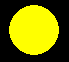
\includegraphics[width=20mm]{good_coin.png} - Dobra moneta \newline

\includegraphics[width=20mm]{bad_coin.png} - Zła moneta\newline
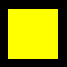
\includegraphics[width=20mm]{exit.png} - Cel. Jeżeli gracz tu dotrze epizod się kończy a gra rozpoczyna się od nowa\newline

\subsection{Reprezentacja stanu gry}

Stan gry przechowywany jest jako tabela dwuwymiarowa zawierająca liczby naturalne. Każda liczba reprezentuje obiekt na planszy. Puste pole oznaczane jest jako 0, monety oznaczane są liczbami 1-9 w zależności od ich wartości, podobnie złe monety od 11-19, wyjście jako 20, gracz 21. Przykładowa plansza 3x3 może więc wyglądać tak:

\begin{center}
\begin{tabular}{ |c|c|c| }
\hline
20 & 0 & 5 \\
\hline
0 & 0 & 0 \\
\hline
15 & 0 & 21 \\
\hline
\end{tabular}
\newline
\end{center} 

Odpowiada to takiemu stanowi planszy:

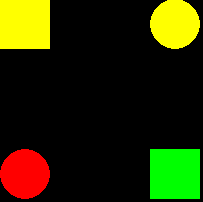
\includegraphics[width=45mm]{przyklad3.png}

\subsection{Implementacja Q-Tabeli}

Najpierw zajmiemy się stworzeniem Q-Tabeli. Przypomnijmy sobie szablon jak powinna ona wyglądać:

\begin{center}
\begin{tabular}{ |c|c|c|c|c| }
\hline
Stan /  Akcja & Akcja 1 & Akcja 2 & Akcja 3 & Akcja 4 \\
\hline
Stan 1 & \small{0} & \small{0} & \small{0} & \small{0} \\
\hline
Stan 2 & \small{0} & \small{0} & \small{0} & \small{0} \\
\hline
Stan 3 & \small{0} & \small{0} & \small{0} & \small{0} \\
\hline
Stan 4 & \small{0} & \small{0} & \small{0} & \small{0} \\
\hline
Stan 5 & \small{0} & \small{0} & \small{0} & \small{0} \\
\hline 
\end{tabular}
\newline \newline
\end{center} 
 W tym momencie napotkujemy problem. Nasze stany to tablice dwuwymiarowe, a nie liczby naturalne, które mogą służyć za wartości w tabeli ospowiadające Stan 1, Stan 2 itd. Czy nie byłoby wygodniej gdybyśmy mogli przedstawić stan gry, czyli tablicę dwuwymairową jako liczbę naturalną? Otóż jest na to pewien sposób. Wykorzystamy fakt że w tablicy przechowujemy jedynie liczby naturalne. Wyobraźmy sobie, że zamieniamy tę tablicę 2-wymiarową na 1-wymiarową, ustawiając kolejne rzędy obok siebie:
\newline \newline Taką tablicę
\begin{center}
\begin{tabular}{ |c|c|c| }
\hline
20 & 0 & 5 \\
\hline
0 & 0 & 0 \\
\hline
15 & 0 & 21 \\
\hline
\end{tabular}
\end{center} 
Zamieniamy w taką
\begin{center}
\begin{tabular}{ |c|c|c|c|c|c|c|c|c| }
\hline
20 & 0 & 5 & 0 & 0 & 0 & 15 & 0 & 21 \\
\hline
\end{tabular}
\newline
\end{center} 

Teraz potraktujmy to jako jedną dużą liczbę. Ale chwila, nie możemy uznać kolejnych komórek za cyfry, są w nich elementy większe od 9. Tak, ale nikt nie powiedział że ta liczba musi być w systemie dziesiętnym! Weźmy największą wartość w tej tablicy i załóżmy że działamy w systemie liczbowym o 1 większym od niej. (tutaj 22). Teraz potraktujmy tę tablicę jako jedną liczbę w tym systemie, gdzie kolejne komórko odpowiadają cyfrom w systemie o podstawie 22. Nastepnie obliczamy wartość tej liczby w systemie dziesiętnym i mamy naszą unikalną liczbę naturalną reprezentującą stan gry. Dla powyższej tablicy jest to:
\[20*22^8 + 5*22^6 + 15*22^2 + 21 = 1098084377521\]
W ten sposób uzało nam się przedstawić tablicę dwuwymiarową reprezentującą stan gry jako liczbę naturalną! Tak, jest to duża liczba, ale na szczęście komputery mają to do siebie że dobrze radzą sobie z dużymi liczbami, a zwłaszcza ich mnożeniem i dodawaniem.
\newline \newline Skąd jednak wiemy, że ta liczba jest unikalna? Czy mamy pewność, nie będzie jakiegoś innego ustawienia planszy, które da ten sam wynik? Cóż, liczby naturalne w dowolnym systemie są równe, wtedy i tylko wtedy gdy ich cyfry na kolejnych pozycjach są równe. Oznacza to że każda plansza reprezentuje unikalną liczbę w systemie 22-kowym. Można również łatwo zauważyć, że każda liczba w systemie o podstawie 22 odpowiada dokładnie jednej liczbie w systemie dziesiętnym. Można powiedzieć że funkcja zamieniająca liczby naturalne z systemu o podstawie 22 na system o podstawie 10 jest bijekcją.
\newline \newline Nie będziemy oczywiście tworzyć tabeli która ma miliardy indeksów. Zamiast tego użyjemy mapy haszującej. Przypisuje ona pewnemu kluczowi jakąś konkretną wartość. W naszym przypadku kluczem będzie para (stan, akcja). Stan przedstawiamy sposobem opisanym powyżej. Akcjami jest krok w górę, prawo, dół lub lewo. Oznaczamy je odpowienio liczbami \(0, 1, 2, 3\)
Na przykład, dla naszej planszy:
\begin{center}
\begin{tabular}{ |c|c|c| }
\hline
20 & 0 & 5 \\
\hline
0 & 0 & 0 \\
\hline
15 & 0 & 21 \\
\hline
\end{tabular}
\end{center} 
Jeżeli w tym stanie zrobienie kroku w górę byłoby warte 7 punktów, w naszej mapie haszującej reprezentującą Q-Tabelę wyglądałoby to tak:
\[\{ (1098084377521, 0) : 7 \}\]
A co jeżeli chcemy odczytać wartośc której jeszcze w mapie nie ma? Z definicji wszystkie wartości w Q-Tabeli są inicjalizowane na 0, więc wtedy po prostu zwracamy 0.
\newline \newline Podsumowując, jeżeli chcielibyśmy wpisać do Q-Tablei wartość W1 w polu (Stan 1, Akcja 1), to najpierw zamieniamy ten stan na liczbę naturalną S1 wcześniej przedstawionym sposobem, Akcję 1 na liczbę A1 od 0 do 3 w zależności od Akcji, po czym zapisujemy element \{(S1, A1) :  W1\} do mapy haszującej reprezentującej Q-Tabelę.

\subsection{Nagrody}

Agent otrzymuje nagrodę lub karę po wykonaniu ruchu w zależności na jake pole wejdzie. Wartości nagród to:
\newline Dobra moneta:  100 do 900 punktów
\newline Zła moneta: -100 do -900 punktów
\newline Cel: 1000 punktów
\newline \newline A ile punktów powinien dostawać agent za wejście na puste pole? Możnaby pomyśleć że 0. Nie jest to jednak idealne rozwiązanie. Dlaczego? W pewnych sytuacjach prowadzi to do trwania epizodu w nieskończoność. Weźmy dla przykładu taką sytuację: \newline
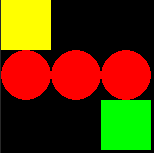
\includegraphics{przyklad4.png} \newline
Załóżmy przez chwilę, że cel ma mniejszą nagrodę niż zła moneta karę. Tutaj agent powinien zebrać jedną złą monetę aby dojść do wyjścia, pomimo faktu że straci punkty, gdyż dojście do wyjścia jest ostatecznym celem gry. Co jednak się stanie? Agent będzie chodził w dolnym wierszu w prawo i lewo w nieskończoność. Dlaczego? Jeżeli nagroda za wejście na puste pole wynosi 0, to chodząc cały czas na puste pola, suma nagród będzie ciągle wynosić 0. Jest to więcej niż nagroda jaką dostałby za zebranie złej monety i dojście do celu.
\newline Co się stanie jednak, jeżeli za wejście na puste pole damy karę -1 punkt? Wtedy chodzenie w nieskończoność na puste pola nie będzie już optymalną strategią. Jest to dlatego, ponieważ z każdym krokiem tracimy 1 punkt. W końcu suma tych straconych punktów będzie większa od punktów które stracilibyśmy idąc do celu. Można to sobie wyobrazić tak jakby agent chodził po rozgrzanych węglach lub po zbitym szkle. Będzie wolał stracić punkty teraz i skończyć epizod, niż tracić powoli punkty w nieskończoność.

\subsection{Program w całości}

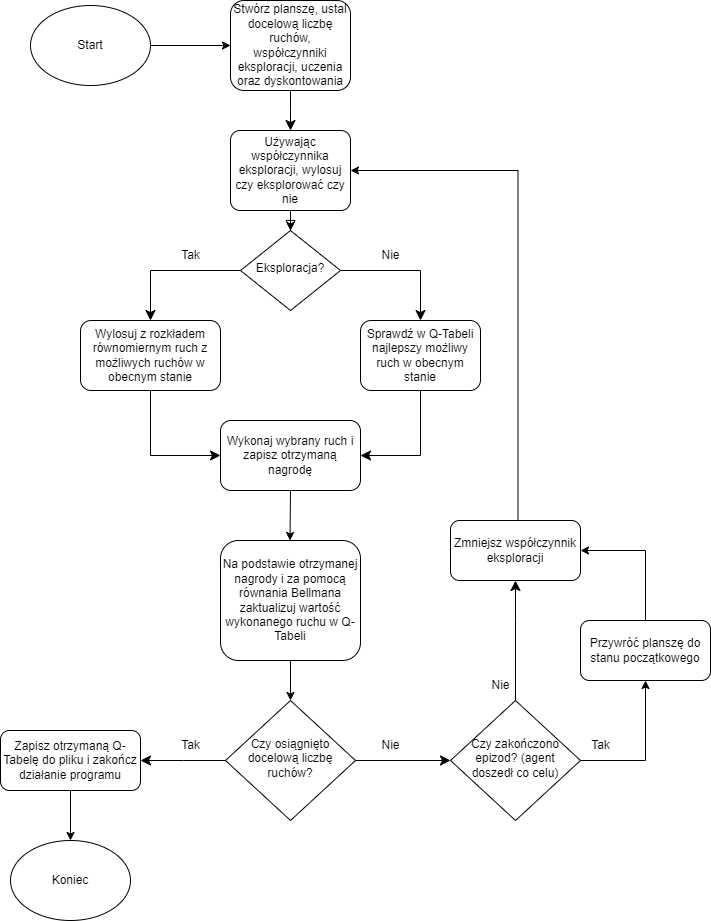
\includegraphics[scale=0.6]{flowchart.png}

\section{Wyniki}

Przestawienie wyników działania algorytmu, wykresy pokazujące działanie i postępy w wynikach na różnych mapach startowych. Przedstawienie wpływu parametrów takich jak współczynnik uczenia i współczynnik eksploracji na skutecznośc uczenia.

Teraz jak wiemy już jak działa algorytm nauczania przez wzmacnianie oraz gra na której będziemy go testować, sprawdźmy jego skuteczność, zaczynając od prostych poziomów.
\newline 
\newline Plansza 1
\newline Liczba ruchów = 20000
\newline \(\alpha = 0.95\)
\newline \(\gamma = 0.99\)
\newline \(\epsilon_{start} = 1\)
\newline \(\epsilon_{koniec} = 0.01\) \newline

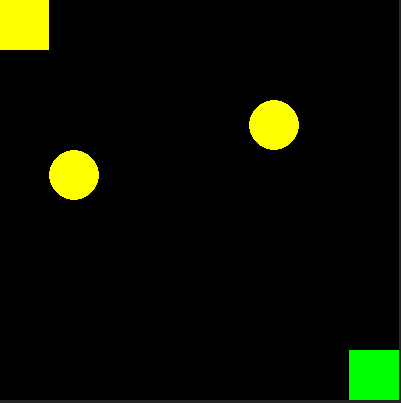
\includegraphics[scale=0.8]{testy/plansza1.png} \newline
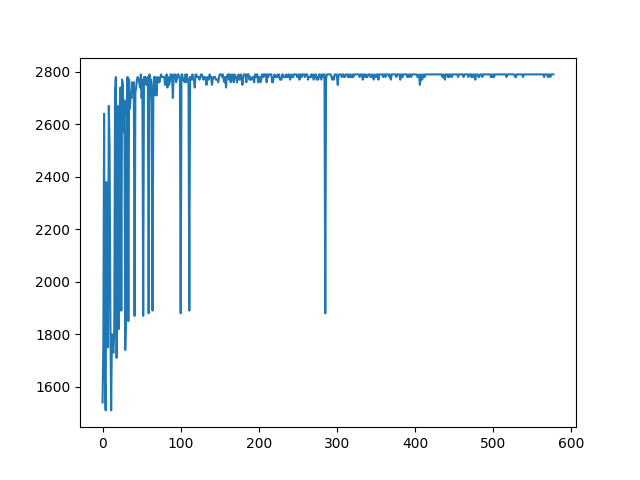
\includegraphics[scale=0.8]{testy/wykres1.png}



\section{Podsumowanie i zastosowania}

Uczenie przez ma wiele zastosowań, poza nauką w gry przedstawioną w tej pracy. Stosuje się ją to tworzenia algorytmów.

 Jakieś adekwatne podsumowanie, dlaczego wybrałem ten temat, jak można dalej ulepszać zaprezentowany algorytm (Deep Q-Learning, Double Deep Q-Learning).




\end{document}